\documentclass[11pt]{article}

    \usepackage[breakable]{tcolorbox}
    \usepackage{parskip} % Stop auto-indenting (to mimic markdown behaviour)
    
    \usepackage{iftex}
    \ifPDFTeX
    	\usepackage[T1]{fontenc}
    	\usepackage{mathpazo}
    \else
    	\usepackage{fontspec}
    \fi

    % Basic figure setup, for now with no caption control since it's done
    % automatically by Pandoc (which extracts ![](path) syntax from Markdown).
    \usepackage{graphicx}
    % Maintain compatibility with old templates. Remove in nbconvert 6.0
    \let\Oldincludegraphics\includegraphics
    % Ensure that by default, figures have no caption (until we provide a
    % proper Figure object with a Caption API and a way to capture that
    % in the conversion process - todo).
    \usepackage{caption}
    \DeclareCaptionFormat{nocaption}{}
    \captionsetup{format=nocaption,aboveskip=0pt,belowskip=0pt}

    \usepackage{float}
    \floatplacement{figure}{H} % forces figures to be placed at the correct location
    \usepackage{xcolor} % Allow colors to be defined
    \usepackage{enumerate} % Needed for markdown enumerations to work
    \usepackage{geometry} % Used to adjust the document margins
    \usepackage{amsmath} % Equations
    \usepackage{amssymb} % Equations
    \usepackage{physics}
    \usepackage{textcomp} % defines textquotesingle
    % Hack from http://tex.stackexchange.com/a/47451/13684:
    \AtBeginDocument{%
        \def\PYZsq{\textquotesingle}% Upright quotes in Pygmentized code
    }
    \usepackage{upquote} % Upright quotes for verbatim code
    \usepackage{eurosym} % defines \euro
    \usepackage[mathletters]{ucs} % Extended unicode (utf-8) support
    \usepackage{fancyvrb} % verbatim replacement that allows latex
    \usepackage{grffile} % extends the file name processing of package graphics 
                         % to support a larger range
    \makeatletter % fix for old versions of grffile with XeLaTeX
    \@ifpackagelater{grffile}{2019/11/01}
    {
      % Do nothing on new versions
    }
    {
      \def\Gread@@xetex#1{%
        \IfFileExists{"\Gin@base".bb}%
        {\Gread@eps{\Gin@base.bb}}%
        {\Gread@@xetex@aux#1}%
      }
    }
    \makeatother
    \usepackage[Export]{adjustbox} % Used to constrain images to a maximum size
    \adjustboxset{max size={0.9\linewidth}{0.9\paperheight}}

    % The hyperref package gives us a pdf with properly built
    % internal navigation ('pdf bookmarks' for the table of contents,
    % internal cross-reference links, web links for URLs, etc.)
    \usepackage{hyperref}
    % The default LaTeX title has an obnoxious amount of whitespace. By default,
    % titling removes some of it. It also provides customization options.
    \usepackage{titling}
    \usepackage{longtable} % longtable support required by pandoc >1.10
    \usepackage{booktabs}  % table support for pandoc > 1.12.2
    \usepackage[inline]{enumitem} % IRkernel/repr support (it uses the enumerate* environment)
    \usepackage[normalem]{ulem} % ulem is needed to support strikethroughs (\sout)
                                % normalem makes italics be italics, not underlines
    \usepackage{mathrsfs}

    \usepackage[version=4,arrows=pgf-filled,
textfontname=sffamily,
mathfontname=mathsf]{mhchem}
    

    
    % Colors for the hyperref package
    \definecolor{urlcolor}{rgb}{0,.145,.698}
    \definecolor{linkcolor}{rgb}{.71,0.21,0.01}
    \definecolor{citecolor}{rgb}{.12,.54,.11}

    % ANSI colors
    \definecolor{ansi-black}{HTML}{3E424D}
    \definecolor{ansi-black-intense}{HTML}{282C36}
    \definecolor{ansi-red}{HTML}{E75C58}
    \definecolor{ansi-red-intense}{HTML}{B22B31}
    \definecolor{ansi-green}{HTML}{00A250}
    \definecolor{ansi-green-intense}{HTML}{007427}
    \definecolor{ansi-yellow}{HTML}{DDB62B}
    \definecolor{ansi-yellow-intense}{HTML}{B27D12}
    \definecolor{ansi-blue}{HTML}{208FFB}
    \definecolor{ansi-blue-intense}{HTML}{0065CA}
    \definecolor{ansi-magenta}{HTML}{D160C4}
    \definecolor{ansi-magenta-intense}{HTML}{A03196}
    \definecolor{ansi-cyan}{HTML}{60C6C8}
    \definecolor{ansi-cyan-intense}{HTML}{258F8F}
    \definecolor{ansi-white}{HTML}{C5C1B4}
    \definecolor{ansi-white-intense}{HTML}{A1A6B2}
    \definecolor{ansi-default-inverse-fg}{HTML}{FFFFFF}
    \definecolor{ansi-default-inverse-bg}{HTML}{000000}

    % common color for the border for error outputs.
    \definecolor{outerrorbackground}{HTML}{FFDFDF}

    % commands and environments needed by pandoc snippets
    % extracted from the output of `pandoc -s`
    \providecommand{\tightlist}{%
      \setlength{\itemsep}{0pt}\setlength{\parskip}{0pt}}
    \DefineVerbatimEnvironment{Highlighting}{Verbatim}{commandchars=\\\{\}}
    % Add ',fontsize=\small' for more characters per line
    \newenvironment{Shaded}{}{}
    \newcommand{\KeywordTok}[1]{\textcolor[rgb]{0.00,0.44,0.13}{\textbf{{#1}}}}
    \newcommand{\DataTypeTok}[1]{\textcolor[rgb]{0.56,0.13,0.00}{{#1}}}
    \newcommand{\DecValTok}[1]{\textcolor[rgb]{0.25,0.63,0.44}{{#1}}}
    \newcommand{\BaseNTok}[1]{\textcolor[rgb]{0.25,0.63,0.44}{{#1}}}
    \newcommand{\FloatTok}[1]{\textcolor[rgb]{0.25,0.63,0.44}{{#1}}}
    \newcommand{\CharTok}[1]{\textcolor[rgb]{0.25,0.44,0.63}{{#1}}}
    \newcommand{\StringTok}[1]{\textcolor[rgb]{0.25,0.44,0.63}{{#1}}}
    \newcommand{\CommentTok}[1]{\textcolor[rgb]{0.38,0.63,0.69}{\textit{{#1}}}}
    \newcommand{\OtherTok}[1]{\textcolor[rgb]{0.00,0.44,0.13}{{#1}}}
    \newcommand{\AlertTok}[1]{\textcolor[rgb]{1.00,0.00,0.00}{\textbf{{#1}}}}
    \newcommand{\FunctionTok}[1]{\textcolor[rgb]{0.02,0.16,0.49}{{#1}}}
    \newcommand{\RegionMarkerTok}[1]{{#1}}
    \newcommand{\ErrorTok}[1]{\textcolor[rgb]{1.00,0.00,0.00}{\textbf{{#1}}}}
    \newcommand{\NormalTok}[1]{{#1}}
    
    % Additional commands for more recent versions of Pandoc
    \newcommand{\ConstantTok}[1]{\textcolor[rgb]{0.53,0.00,0.00}{{#1}}}
    \newcommand{\SpecialCharTok}[1]{\textcolor[rgb]{0.25,0.44,0.63}{{#1}}}
    \newcommand{\VerbatimStringTok}[1]{\textcolor[rgb]{0.25,0.44,0.63}{{#1}}}
    \newcommand{\SpecialStringTok}[1]{\textcolor[rgb]{0.73,0.40,0.53}{{#1}}}
    \newcommand{\ImportTok}[1]{{#1}}
    \newcommand{\DocumentationTok}[1]{\textcolor[rgb]{0.73,0.13,0.13}{\textit{{#1}}}}
    \newcommand{\AnnotationTok}[1]{\textcolor[rgb]{0.38,0.63,0.69}{\textbf{\textit{{#1}}}}}
    \newcommand{\CommentVarTok}[1]{\textcolor[rgb]{0.38,0.63,0.69}{\textbf{\textit{{#1}}}}}
    \newcommand{\VariableTok}[1]{\textcolor[rgb]{0.10,0.09,0.49}{{#1}}}
    \newcommand{\ControlFlowTok}[1]{\textcolor[rgb]{0.00,0.44,0.13}{\textbf{{#1}}}}
    \newcommand{\OperatorTok}[1]{\textcolor[rgb]{0.40,0.40,0.40}{{#1}}}
    \newcommand{\BuiltInTok}[1]{{#1}}
    \newcommand{\ExtensionTok}[1]{{#1}}
    \newcommand{\PreprocessorTok}[1]{\textcolor[rgb]{0.74,0.48,0.00}{{#1}}}
    \newcommand{\AttributeTok}[1]{\textcolor[rgb]{0.49,0.56,0.16}{{#1}}}
    \newcommand{\InformationTok}[1]{\textcolor[rgb]{0.38,0.63,0.69}{\textbf{\textit{{#1}}}}}
    \newcommand{\WarningTok}[1]{\textcolor[rgb]{0.38,0.63,0.69}{\textbf{\textit{{#1}}}}}
    
    
    % Define a nice break command that doesn't care if a line doesn't already
    % exist.
    \def\br{\hspace*{\fill} \\* }
    % Math Jax compatibility definitions
    \def\gt{>}
    \def\lt{<}
    \let\Oldtex\TeX
    \let\Oldlatex\LaTeX
    \renewcommand{\TeX}{\textrm{\Oldtex}}
    \renewcommand{\LaTeX}{\textrm{\Oldlatex}}
    % Document parameters
    % Document title
    \title{PC3233 Assignment 4}
    
    
    
    
    
% Pygments definitions
\makeatletter
\def\PY@reset{\let\PY@it=\relax \let\PY@bf=\relax%
    \let\PY@ul=\relax \let\PY@tc=\relax%
    \let\PY@bc=\relax \let\PY@ff=\relax}
\def\PY@tok#1{\csname PY@tok@#1\endcsname}
\def\PY@toks#1+{\ifx\relax#1\empty\else%
    \PY@tok{#1}\expandafter\PY@toks\fi}
\def\PY@do#1{\PY@bc{\PY@tc{\PY@ul{%
    \PY@it{\PY@bf{\PY@ff{#1}}}}}}}
\def\PY#1#2{\PY@reset\PY@toks#1+\relax+\PY@do{#2}}

\@namedef{PY@tok@w}{\def\PY@tc##1{\textcolor[rgb]{0.73,0.73,0.73}{##1}}}
\@namedef{PY@tok@c}{\let\PY@it=\textit\def\PY@tc##1{\textcolor[rgb]{0.24,0.48,0.48}{##1}}}
\@namedef{PY@tok@cp}{\def\PY@tc##1{\textcolor[rgb]{0.61,0.40,0.00}{##1}}}
\@namedef{PY@tok@k}{\let\PY@bf=\textbf\def\PY@tc##1{\textcolor[rgb]{0.00,0.50,0.00}{##1}}}
\@namedef{PY@tok@kp}{\def\PY@tc##1{\textcolor[rgb]{0.00,0.50,0.00}{##1}}}
\@namedef{PY@tok@kt}{\def\PY@tc##1{\textcolor[rgb]{0.69,0.00,0.25}{##1}}}
\@namedef{PY@tok@o}{\def\PY@tc##1{\textcolor[rgb]{0.40,0.40,0.40}{##1}}}
\@namedef{PY@tok@ow}{\let\PY@bf=\textbf\def\PY@tc##1{\textcolor[rgb]{0.67,0.13,1.00}{##1}}}
\@namedef{PY@tok@nb}{\def\PY@tc##1{\textcolor[rgb]{0.00,0.50,0.00}{##1}}}
\@namedef{PY@tok@nf}{\def\PY@tc##1{\textcolor[rgb]{0.00,0.00,1.00}{##1}}}
\@namedef{PY@tok@nc}{\let\PY@bf=\textbf\def\PY@tc##1{\textcolor[rgb]{0.00,0.00,1.00}{##1}}}
\@namedef{PY@tok@nn}{\let\PY@bf=\textbf\def\PY@tc##1{\textcolor[rgb]{0.00,0.00,1.00}{##1}}}
\@namedef{PY@tok@ne}{\let\PY@bf=\textbf\def\PY@tc##1{\textcolor[rgb]{0.80,0.25,0.22}{##1}}}
\@namedef{PY@tok@nv}{\def\PY@tc##1{\textcolor[rgb]{0.10,0.09,0.49}{##1}}}
\@namedef{PY@tok@no}{\def\PY@tc##1{\textcolor[rgb]{0.53,0.00,0.00}{##1}}}
\@namedef{PY@tok@nl}{\def\PY@tc##1{\textcolor[rgb]{0.46,0.46,0.00}{##1}}}
\@namedef{PY@tok@ni}{\let\PY@bf=\textbf\def\PY@tc##1{\textcolor[rgb]{0.44,0.44,0.44}{##1}}}
\@namedef{PY@tok@na}{\def\PY@tc##1{\textcolor[rgb]{0.41,0.47,0.13}{##1}}}
\@namedef{PY@tok@nt}{\let\PY@bf=\textbf\def\PY@tc##1{\textcolor[rgb]{0.00,0.50,0.00}{##1}}}
\@namedef{PY@tok@nd}{\def\PY@tc##1{\textcolor[rgb]{0.67,0.13,1.00}{##1}}}
\@namedef{PY@tok@s}{\def\PY@tc##1{\textcolor[rgb]{0.73,0.13,0.13}{##1}}}
\@namedef{PY@tok@sd}{\let\PY@it=\textit\def\PY@tc##1{\textcolor[rgb]{0.73,0.13,0.13}{##1}}}
\@namedef{PY@tok@si}{\let\PY@bf=\textbf\def\PY@tc##1{\textcolor[rgb]{0.64,0.35,0.47}{##1}}}
\@namedef{PY@tok@se}{\let\PY@bf=\textbf\def\PY@tc##1{\textcolor[rgb]{0.67,0.36,0.12}{##1}}}
\@namedef{PY@tok@sr}{\def\PY@tc##1{\textcolor[rgb]{0.64,0.35,0.47}{##1}}}
\@namedef{PY@tok@ss}{\def\PY@tc##1{\textcolor[rgb]{0.10,0.09,0.49}{##1}}}
\@namedef{PY@tok@sx}{\def\PY@tc##1{\textcolor[rgb]{0.00,0.50,0.00}{##1}}}
\@namedef{PY@tok@m}{\def\PY@tc##1{\textcolor[rgb]{0.40,0.40,0.40}{##1}}}
\@namedef{PY@tok@gh}{\let\PY@bf=\textbf\def\PY@tc##1{\textcolor[rgb]{0.00,0.00,0.50}{##1}}}
\@namedef{PY@tok@gu}{\let\PY@bf=\textbf\def\PY@tc##1{\textcolor[rgb]{0.50,0.00,0.50}{##1}}}
\@namedef{PY@tok@gd}{\def\PY@tc##1{\textcolor[rgb]{0.63,0.00,0.00}{##1}}}
\@namedef{PY@tok@gi}{\def\PY@tc##1{\textcolor[rgb]{0.00,0.52,0.00}{##1}}}
\@namedef{PY@tok@gr}{\def\PY@tc##1{\textcolor[rgb]{0.89,0.00,0.00}{##1}}}
\@namedef{PY@tok@ge}{\let\PY@it=\textit}
\@namedef{PY@tok@gs}{\let\PY@bf=\textbf}
\@namedef{PY@tok@gp}{\let\PY@bf=\textbf\def\PY@tc##1{\textcolor[rgb]{0.00,0.00,0.50}{##1}}}
\@namedef{PY@tok@go}{\def\PY@tc##1{\textcolor[rgb]{0.44,0.44,0.44}{##1}}}
\@namedef{PY@tok@gt}{\def\PY@tc##1{\textcolor[rgb]{0.00,0.27,0.87}{##1}}}
\@namedef{PY@tok@err}{\def\PY@bc##1{{\setlength{\fboxsep}{\string -\fboxrule}\fcolorbox[rgb]{1.00,0.00,0.00}{1,1,1}{\strut ##1}}}}
\@namedef{PY@tok@kc}{\let\PY@bf=\textbf\def\PY@tc##1{\textcolor[rgb]{0.00,0.50,0.00}{##1}}}
\@namedef{PY@tok@kd}{\let\PY@bf=\textbf\def\PY@tc##1{\textcolor[rgb]{0.00,0.50,0.00}{##1}}}
\@namedef{PY@tok@kn}{\let\PY@bf=\textbf\def\PY@tc##1{\textcolor[rgb]{0.00,0.50,0.00}{##1}}}
\@namedef{PY@tok@kr}{\let\PY@bf=\textbf\def\PY@tc##1{\textcolor[rgb]{0.00,0.50,0.00}{##1}}}
\@namedef{PY@tok@bp}{\def\PY@tc##1{\textcolor[rgb]{0.00,0.50,0.00}{##1}}}
\@namedef{PY@tok@fm}{\def\PY@tc##1{\textcolor[rgb]{0.00,0.00,1.00}{##1}}}
\@namedef{PY@tok@vc}{\def\PY@tc##1{\textcolor[rgb]{0.10,0.09,0.49}{##1}}}
\@namedef{PY@tok@vg}{\def\PY@tc##1{\textcolor[rgb]{0.10,0.09,0.49}{##1}}}
\@namedef{PY@tok@vi}{\def\PY@tc##1{\textcolor[rgb]{0.10,0.09,0.49}{##1}}}
\@namedef{PY@tok@vm}{\def\PY@tc##1{\textcolor[rgb]{0.10,0.09,0.49}{##1}}}
\@namedef{PY@tok@sa}{\def\PY@tc##1{\textcolor[rgb]{0.73,0.13,0.13}{##1}}}
\@namedef{PY@tok@sb}{\def\PY@tc##1{\textcolor[rgb]{0.73,0.13,0.13}{##1}}}
\@namedef{PY@tok@sc}{\def\PY@tc##1{\textcolor[rgb]{0.73,0.13,0.13}{##1}}}
\@namedef{PY@tok@dl}{\def\PY@tc##1{\textcolor[rgb]{0.73,0.13,0.13}{##1}}}
\@namedef{PY@tok@s2}{\def\PY@tc##1{\textcolor[rgb]{0.73,0.13,0.13}{##1}}}
\@namedef{PY@tok@sh}{\def\PY@tc##1{\textcolor[rgb]{0.73,0.13,0.13}{##1}}}
\@namedef{PY@tok@s1}{\def\PY@tc##1{\textcolor[rgb]{0.73,0.13,0.13}{##1}}}
\@namedef{PY@tok@mb}{\def\PY@tc##1{\textcolor[rgb]{0.40,0.40,0.40}{##1}}}
\@namedef{PY@tok@mf}{\def\PY@tc##1{\textcolor[rgb]{0.40,0.40,0.40}{##1}}}
\@namedef{PY@tok@mh}{\def\PY@tc##1{\textcolor[rgb]{0.40,0.40,0.40}{##1}}}
\@namedef{PY@tok@mi}{\def\PY@tc##1{\textcolor[rgb]{0.40,0.40,0.40}{##1}}}
\@namedef{PY@tok@il}{\def\PY@tc##1{\textcolor[rgb]{0.40,0.40,0.40}{##1}}}
\@namedef{PY@tok@mo}{\def\PY@tc##1{\textcolor[rgb]{0.40,0.40,0.40}{##1}}}
\@namedef{PY@tok@ch}{\let\PY@it=\textit\def\PY@tc##1{\textcolor[rgb]{0.24,0.48,0.48}{##1}}}
\@namedef{PY@tok@cm}{\let\PY@it=\textit\def\PY@tc##1{\textcolor[rgb]{0.24,0.48,0.48}{##1}}}
\@namedef{PY@tok@cpf}{\let\PY@it=\textit\def\PY@tc##1{\textcolor[rgb]{0.24,0.48,0.48}{##1}}}
\@namedef{PY@tok@c1}{\let\PY@it=\textit\def\PY@tc##1{\textcolor[rgb]{0.24,0.48,0.48}{##1}}}
\@namedef{PY@tok@cs}{\let\PY@it=\textit\def\PY@tc##1{\textcolor[rgb]{0.24,0.48,0.48}{##1}}}

\def\PYZbs{\char`\\}
\def\PYZus{\char`\_}
\def\PYZob{\char`\{}
\def\PYZcb{\char`\}}
\def\PYZca{\char`\^}
\def\PYZam{\char`\&}
\def\PYZlt{\char`\<}
\def\PYZgt{\char`\>}
\def\PYZsh{\char`\#}
\def\PYZpc{\char`\%}
\def\PYZdl{\char`\$}
\def\PYZhy{\char`\-}
\def\PYZsq{\char`\'}
\def\PYZdq{\char`\"}
\def\PYZti{\char`\~}
% for compatibility with earlier versions
\def\PYZat{@}
\def\PYZlb{[}
\def\PYZrb{]}
\makeatother


    % For linebreaks inside Verbatim environment from package fancyvrb. 
    \makeatletter
        \newbox\Wrappedcontinuationbox 
        \newbox\Wrappedvisiblespacebox 
        \newcommand*\Wrappedvisiblespace {\textcolor{red}{\textvisiblespace}} 
        \newcommand*\Wrappedcontinuationsymbol {\textcolor{red}{\llap{\tiny$\m@th\hookrightarrow$}}} 
        \newcommand*\Wrappedcontinuationindent {3ex } 
        \newcommand*\Wrappedafterbreak {\kern\Wrappedcontinuationindent\copy\Wrappedcontinuationbox} 
        % Take advantage of the already applied Pygments mark-up to insert 
        % potential linebreaks for TeX processing. 
        %        {, <, #, %, $, ' and ": go to next line. 
        %        _, }, ^, &, >, - and ~: stay at end of broken line. 
        % Use of \textquotesingle for straight quote. 
        \newcommand*\Wrappedbreaksatspecials {% 
            \def\PYGZus{\discretionary{\char`\_}{\Wrappedafterbreak}{\char`\_}}% 
            \def\PYGZob{\discretionary{}{\Wrappedafterbreak\char`\{}{\char`\{}}% 
            \def\PYGZcb{\discretionary{\char`\}}{\Wrappedafterbreak}{\char`\}}}% 
            \def\PYGZca{\discretionary{\char`\^}{\Wrappedafterbreak}{\char`\^}}% 
            \def\PYGZam{\discretionary{\char`\&}{\Wrappedafterbreak}{\char`\&}}% 
            \def\PYGZlt{\discretionary{}{\Wrappedafterbreak\char`\<}{\char`\<}}% 
            \def\PYGZgt{\discretionary{\char`\>}{\Wrappedafterbreak}{\char`\>}}% 
            \def\PYGZsh{\discretionary{}{\Wrappedafterbreak\char`\#}{\char`\#}}% 
            \def\PYGZpc{\discretionary{}{\Wrappedafterbreak\char`\%}{\char`\%}}% 
            \def\PYGZdl{\discretionary{}{\Wrappedafterbreak\char`\$}{\char`\$}}% 
            \def\PYGZhy{\discretionary{\char`\-}{\Wrappedafterbreak}{\char`\-}}% 
            \def\PYGZsq{\discretionary{}{\Wrappedafterbreak\textquotesingle}{\textquotesingle}}% 
            \def\PYGZdq{\discretionary{}{\Wrappedafterbreak\char`\"}{\char`\"}}% 
            \def\PYGZti{\discretionary{\char`\~}{\Wrappedafterbreak}{\char`\~}}% 
        } 
        % Some characters . , ; ? ! / are not pygmentized. 
        % This macro makes them "active" and they will insert potential linebreaks 
        \newcommand*\Wrappedbreaksatpunct {% 
            \lccode`\~`\.\lowercase{\def~}{\discretionary{\hbox{\char`\.}}{\Wrappedafterbreak}{\hbox{\char`\.}}}% 
            \lccode`\~`\,\lowercase{\def~}{\discretionary{\hbox{\char`\,}}{\Wrappedafterbreak}{\hbox{\char`\,}}}% 
            \lccode`\~`\;\lowercase{\def~}{\discretionary{\hbox{\char`\;}}{\Wrappedafterbreak}{\hbox{\char`\;}}}% 
            \lccode`\~`\:\lowercase{\def~}{\discretionary{\hbox{\char`\:}}{\Wrappedafterbreak}{\hbox{\char`\:}}}% 
            \lccode`\~`\?\lowercase{\def~}{\discretionary{\hbox{\char`\?}}{\Wrappedafterbreak}{\hbox{\char`\?}}}% 
            \lccode`\~`\!\lowercase{\def~}{\discretionary{\hbox{\char`\!}}{\Wrappedafterbreak}{\hbox{\char`\!}}}% 
            \lccode`\~`\/\lowercase{\def~}{\discretionary{\hbox{\char`\/}}{\Wrappedafterbreak}{\hbox{\char`\/}}}% 
            \catcode`\.\active
            \catcode`\,\active 
            \catcode`\;\active
            \catcode`\:\active
            \catcode`\?\active
            \catcode`\!\active
            \catcode`\/\active 
            \lccode`\~`\~ 	
        }
    \makeatother

    \let\OriginalVerbatim=\Verbatim
    \makeatletter
    \renewcommand{\Verbatim}[1][1]{%
        %\parskip\z@skip
        \sbox\Wrappedcontinuationbox {\Wrappedcontinuationsymbol}%
        \sbox\Wrappedvisiblespacebox {\FV@SetupFont\Wrappedvisiblespace}%
        \def\FancyVerbFormatLine ##1{\hsize\linewidth
            \vtop{\raggedright\hyphenpenalty\z@\exhyphenpenalty\z@
                \doublehyphendemerits\z@\finalhyphendemerits\z@
                \strut ##1\strut}%
        }%
        % If the linebreak is at a space, the latter will be displayed as visible
        % space at end of first line, and a continuation symbol starts next line.
        % Stretch/shrink are however usually zero for typewriter font.
        \def\FV@Space {%
            \nobreak\hskip\z@ plus\fontdimen3\font minus\fontdimen4\font
            \discretionary{\copy\Wrappedvisiblespacebox}{\Wrappedafterbreak}
            {\kern\fontdimen2\font}%
        }%
        
        % Allow breaks at special characters using \PYG... macros.
        \Wrappedbreaksatspecials
        % Breaks at punctuation characters . , ; ? ! and / need catcode=\active 	
        \OriginalVerbatim[#1,codes*=\Wrappedbreaksatpunct]%
    }
    \makeatother

    % Exact colors from NB
    \definecolor{incolor}{HTML}{303F9F}
    \definecolor{outcolor}{HTML}{D84315}
    \definecolor{cellborder}{HTML}{CFCFCF}
    \definecolor{cellbackground}{HTML}{F7F7F7}
    
    % prompt
    \makeatletter
    \newcommand{\boxspacing}{\kern\kvtcb@left@rule\kern\kvtcb@boxsep}
    \makeatother
    \newcommand{\prompt}[4]{
        {\ttfamily\llap{{\color{#2}[#3]:\hspace{3pt}#4}}\vspace{-\baselineskip}}
    }
    

    
    % Prevent overflowing lines due to hard-to-break entities
    \sloppy 
    % Setup hyperref package
    \hypersetup{
      breaklinks=true,  % so long urls are correctly broken across lines
      colorlinks=true,
      urlcolor=urlcolor,
      linkcolor=linkcolor,
      citecolor=citecolor,
      }
    % Slightly bigger margins than the latex defaults
    
    \geometry{verbose,tmargin=1in,bmargin=1in,lmargin=1in,rmargin=1in}
    
    

\begin{document}
    
    \maketitle
    
    \section{Dipole-Dipole Interaction}
    \subsection{Part A}

    The interaction energy, $E$, between two magnetic dipole, $\vec{\mu}_1$ and $\vec{\mu}_2$, is given by:

    \begin{equation}
      E = + \frac{\mu_0}{4\pi} \frac{\vec{\mu}_1 \cdot \vec{\mu}_2 - 3(\vec{\mu}_1 \cdot \hat{r})(\vec{\mu}_2 \cdot \hat{r})}{r^3}
    \end{equation}

    Since the energy is magnetic potential energy is given by:

    \begin{equation}
      E = - \vec{mu} \cdot \vec{B}
    \end{equation}

    Therefore, we can extract the magnetic field of magnetic dipole, $\vec{B_i}$, from the interaction energy, $E$:

    \begin{equation}
      \vec{B_i(r)} = - \frac{\mu_0}{4\pi} \frac{3(\vec{\mu}_i \cdot \vec{r})\vec{r}}{r^5} - \frac{\vec{\mu}_i}{r^3}
    \end{equation}

    Hence, in order for $E = 0$ for any given $|\vec{r}|$, $B_i$ must be orthornormal to $\vec{\mu_j}$.

  \subsection{Part B}

  For parallel moments, we can expand the dot product of $E$ as:

  \begin{equation}
    E = \frac{\mu_0}{4\pi} \frac{\mu_1 \mu_2}{r^3} (1 - 3 \cos^2 \theta)
  \end{equation}

  Then, we can obtain the following:
  \begin{equation}
    \begin{cases}
      \displaystyle
      E_{min} = -\frac{\mu_0}{2\pi} \frac{\mu_1 \mu_2}{r^3} & \text{if } \theta = 0, \pi \\
      \\
      \displaystyle
      E_{max} = +\frac{\mu_0}{4\pi} \frac{\mu_1 \mu_2}{r^3} & \text{if } \theta = \frac{\pi}{2}\\
    \end{cases}
  \end{equation}

  \subsection{Part C}

  For case (b) with $|\vec{r}| = 2\text{\AA}$. We can calculate the interaction energy, $E$, as follows using the 
  formula we obtain from the previous section:

  For electron-electron case, we have:

  \begin{equation}
    \begin{cases}
      \displaystyle
      E_{min} = -\frac{\mu_0}{2\pi} \frac{\mu_B^2}{r^3} = - 6.4505 \times 10^{-24} \text{J} & \text{if } \theta = 0, \pi \\
      \\
      \displaystyle
      E_{max} = +\frac{\mu_0}{4\pi} \frac{\mu_B^2}{r^3} = 3.22527 \times 10^{-24} \text{J} & \text{if } \theta = \frac{\pi}{2}\\
    \end{cases}
  \end{equation}

  For proton-proton case ($\mu_{proton} = 1.4 \times 10^{-26}$ \AA$m^2$), we have:

  \begin{equation}
    \begin{cases}
      \displaystyle
      E_{min} = -\frac{\mu_0}{2\pi} \frac{\mu_{proton}^2}{r^3} = -4.90 \times 10^{-30} \text{J} & \text{if } \theta = 0, \pi \\
      \\
      \displaystyle
      E_{max} = +\frac{\mu_0}{4\pi} \frac{\mu_{proton}^2}{r^3} = 2.45 \times 10^{-30} \text{J} & \text{if } \theta = \frac{\pi}{2}\\
    \end{cases}
  \end{equation}

  To compute the magnetic field, $\vec{B}$, we can rearranged the formula we obtained in part (a):

  \begin{align*}
    E = - \vec{\mu} \cdot \vec{B} &\implies E  = - |\mu| |B| \cos{\theta} \\
    &\implies |B| = \frac{E}{|\mu|} \hspace{0.5in} \text{since $\mu$ always align to the $\vec{B}$} \\
  \end{align*}

  Hence, we can compute the magnetic field, $B$, for the electron-electron as follows:

  \begin{equation}
    \begin{cases}
      \displaystyle
      |B| = \frac{E}{|\mu|} = 0.4016 \text{T} & \text{if } \theta = 0, \pi \\
      \\
      \displaystyle
      |B| = \frac{E}{|\mu|} = 0.2007 \text{T} & \text{if } \theta = \frac{\pi}{2}\\
    \end{cases}
  \end{equation}

  For proton-proton case, we have:

  \begin{equation}
    \begin{cases}
      \displaystyle
      |B| = \frac{E}{|\mu|} = 3.5 \times 10^{-4} \text{T} & \text{if } \theta = 0, \pi \\
      \\
      \displaystyle
      |B| = \frac{E}{|\mu|} = 1.75 \times 10^{-4} \text{T} & \text{if } \theta = \frac{\pi}{2}\\
    \end{cases}
  \end{equation}

  \subsection{Part D}

  Express the interaction energy, $E$, in the previous section in terms of J, $cm^{-1}$, and $\mu K$.

  For electron-electron case, we have:

  \begin{equation}
    \begin{cases}
      \displaystyle
      E_{min} = -\frac{\mu_0}{2\pi} \frac{\mu_B^2}{r^3} = - 6.4505 \times 10^{-24} \text{J} = - 32.47 \text{cm}^{-1} = - 467211 \mu K & \text{if } \theta = 0, \pi \\
      \\
      \displaystyle
      E_{max} = +\frac{\mu_0}{4\pi} \frac{\mu_B^2}{r^3} = 3.22527 \times 10^{-24} \text{J} = 16.24 \text{cm}^{-1} = 233605 \mu K & \text{if } \theta = \frac{\pi}{2}\\
    \end{cases}
  \end{equation}

  For proton-proton case, we have:

  \begin{equation}
    \begin{cases}
      \displaystyle
      E_{min} = -\frac{\mu_0}{2\pi} \frac{\mu_{proton}^2}{r^3} = -4.90 \times 10^{-30} \text{J} = -2.4667 \text{cm}^{-1} = -0.355 \mu K & \text{if } \theta = 0, \pi \\
      \\
      \displaystyle
      E_{max} = +\frac{\mu_0}{4\pi} \frac{\mu_{proton}^2}{r^3} = 2.45 \times 10^{-30} \text{J} = 1.2334 \text{cm}^{-1} = 0.177 \mu K & \text{if } \theta = \frac{\pi}{2}\\
    \end{cases}
  \end{equation}

  \section{Mathematical Relationships}

  Consider the following matrix:

  \begin{equation}
    M = 
    \begin{pmatrix}
      a & b \\
      c & d \\
    \end{pmatrix}
  \end{equation}

  \subsection{Analytic Expression of Eigenvalues}

  To diagonalize the matrix, we solve for the eigenvalues, $\lambda$, by solving the following equation:

  \begin{equation}
    \det(M - \lambda I) = 0
  \end{equation}

  Then, we have:

  \begin{align*}
    \det
    \begin{pmatrix}
      a - \lambda & b \\
      c & d - \lambda \\
    \end{pmatrix}
    &= 0 \\
  \end{align*}

  Then compute the determinant:

  \begin{align*}
    (a - \lambda)(d - \lambda) - bc &= 0\\
    \lambda^2 - (a + d)\lambda + ad - bc &= 0
  \end{align*}

  Since the eigenvalues are the roots of the characteristic equation, which is quadratic, we get
  the analytic expression for $\lambda$ using the quadratic formula:

  \begin{equation}
    \lambda = \frac{-(a + d) \pm \sqrt{(a + d)^2 - 4(ad - bc)}}{2}
  \end{equation}

  \subsection{Generalized $n \times n$ Eignevalues}

  The degree of polynomial of the characteristic equation is $n$, where $n$ 
  is the dimension of the matrix. 

  According to Abel-Ruffini theorem, there is no general solution for the roots of a polynomial of degree $n \geq 5$.

  For degree $n = 2, 3, 4$, we can solve for the roots of the characteristic equation using the quadratic, 
  cubic, and quartic formulae respectively.

  \section{Atoms in Magnetic Field}

  \subsection{Part A}

  Given a \ce{Li^{++}} with $I = 1$. The energy levels due to fine structure splitting is given by:

  \begin{equation}
    E_{n,j} = E_n [1 + \frac{Z^2 \alpha^2}{n}(\frac{1}{j+\frac{1}{2}} - \frac{3}{4n})]
  \end{equation}

  Hence we can determeine the following:

  \begin{equation}
    \begin{cases}
      \displaystyle
      E_{1,\frac{1}{2}} &= E_1 [1 + \frac{Z^2 \alpha^2}{4}] \\
      \\
      \displaystyle
      E_{2,\frac{1}{2}} &= E_2 [1 + \frac{5Z^2 \alpha^2}{16}] \\
      \\
      \displaystyle
      E_{2,\frac{3}{2}} &= E_3 [1 + \frac{Z^2 \alpha^2}{16}] \\
    \end{cases}
  \end{equation}

  The energy levels shift due to Hyperfine strucutre is given by:

  \begin{equation}
    \Delta H_{HF} = \frac{g_i \mu_k B}{2 \sqrt{j(j+1)}}[F(F+1) - I(I+1) - j(j+1)]
  \end{equation}

  The possible of value of total angular mmomentum, is given by:

  \begin{equation}
    F = |j-I|, |j-I+1|, \ldots, |j+I|
  \end{equation}

  Hence, by setting $g_i \mu_k B = 1$, we can compute the energy levels shift due to hyperfine structure.

  \begin{equation}
    \begin{cases}
      \displaystyle
      \Delta H_{HF} = \frac{-2\sqrt{3}}{3} & \text{if } F = \frac{1}{2}, j = \frac{1}{2}, 1s \\
      \\
      \displaystyle
      \Delta H_{HF} = \frac{2\sqrt{6}}{3} & \text{if } F = \frac{3}{2}, j = \frac{1}{2}, 1s \\
      \\
      \displaystyle
      \Delta H_{HF} = -\frac{2\sqrt{3}}{3} & \text{if } F = \frac{1}{2}, j = \frac{1}{2}, 2s \\
      \\
      \displaystyle
      \Delta H_{HF} = \frac{\sqrt{3}}{3} & \text{if } F = \frac{3}{2}, j = \frac{1}{2}, 2s \\
      \\
      \displaystyle
      \Delta H_{HF} = -\frac{\sqrt{15}}{3} & \text{if } F = \frac{1}{2}, j = \frac{3}{2}, 2p \\
      \\
      \displaystyle
      \Delta H_{HF} = \frac{2\sqrt{15}}{15} & \text{if } F = \frac{3}{2}, j = \frac{3}{2}, 2p \\
      \\
      \displaystyle
      \Delta H_{HF} = -\frac{\sqrt{15}}{5} & \text{if } F = \frac{5}{2}, j = \frac{3}{2}, 2p \\
    \end{cases}
  \end{equation}

  Hence we can draw the energy level diagram for the fine and hyperfine structure states as below.

  \begin{figure}[h!]
    \centering
    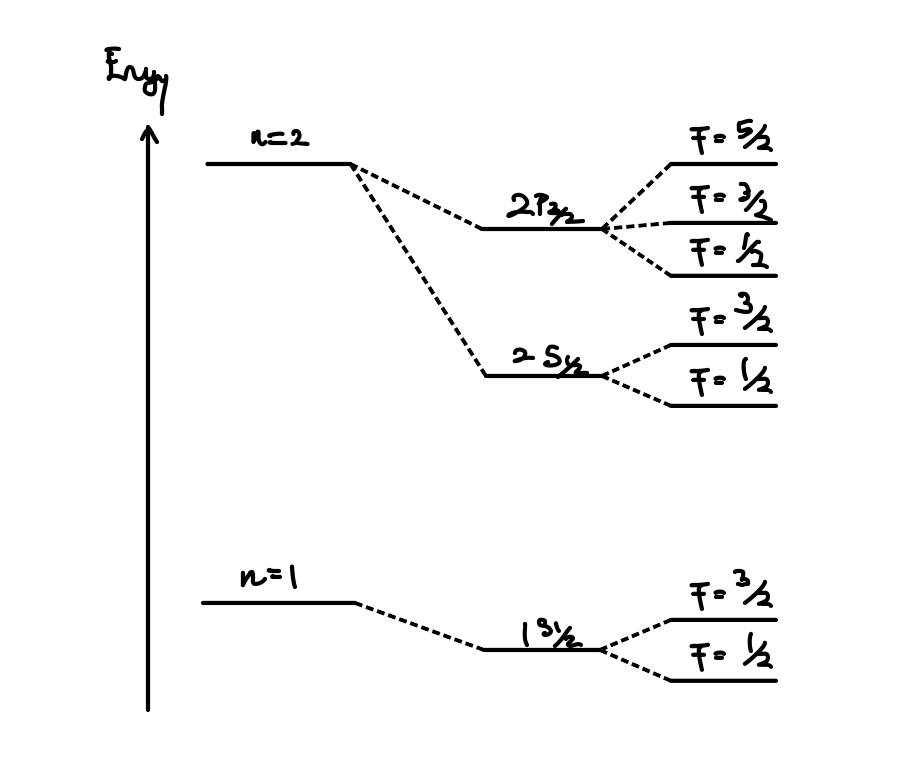
\includegraphics[width=5in]{./image/HyperfineStructure_EnergyLevel.jpg}
  \end{figure}

  \subsection{Part B: Compute Lande Factor}

  For Lande factor, $g_j$, is given by:

  \begin{equation}
    g_j = 1 + \frac{j(j + 1) - l(l + 1) + s(s + 1)}{2j(j + 1)}
  \end{equation}

  Hence, for $g_j$ for all fine structure states up to $n = 2$ is given in the below:

  \begin{equation}
    \begin{cases}
      \displaystyle
      g_j = \frac{1}{3  } & \text{if } j = \frac{1}{2}, l = 1, s = \frac{1}{2} \\
      \\
      \displaystyle
      g_j = \frac{4}{3} & \text{if } j = \frac{3}{2}, l = 1, s = \frac{1}{2} \\
    \end{cases}
  \end{equation}

  \subsection{Part C: Zeeman Effect}

  The Zeeman effect energy splitting, $\Delta E$, is given by:  

  \begin{equation}
    \Delta E = \mu_j g_j \mu_B B
  \end{equation}

  Hence for lowest Zeeman states, we have:

  \begin{equation}
    \Delta E = m_j g_j \mu_B B = \Delta m_j \frac{1}{3} \mu_B B = 1.0304 \times 10^{-24} \text{J}
  \end{equation}


  

  
\end{document}
